\documentclass[tikz, border=10pt]{standalone}
\usepackage[utf8]{inputenc}
\usepackage[T1]{fontenc}
\usepackage{lmodern}
\usepackage{amsmath, amssymb}
\usetikzlibrary{positioning, calc, backgrounds, shapes.geometric, arrows.meta}

\begin{document}

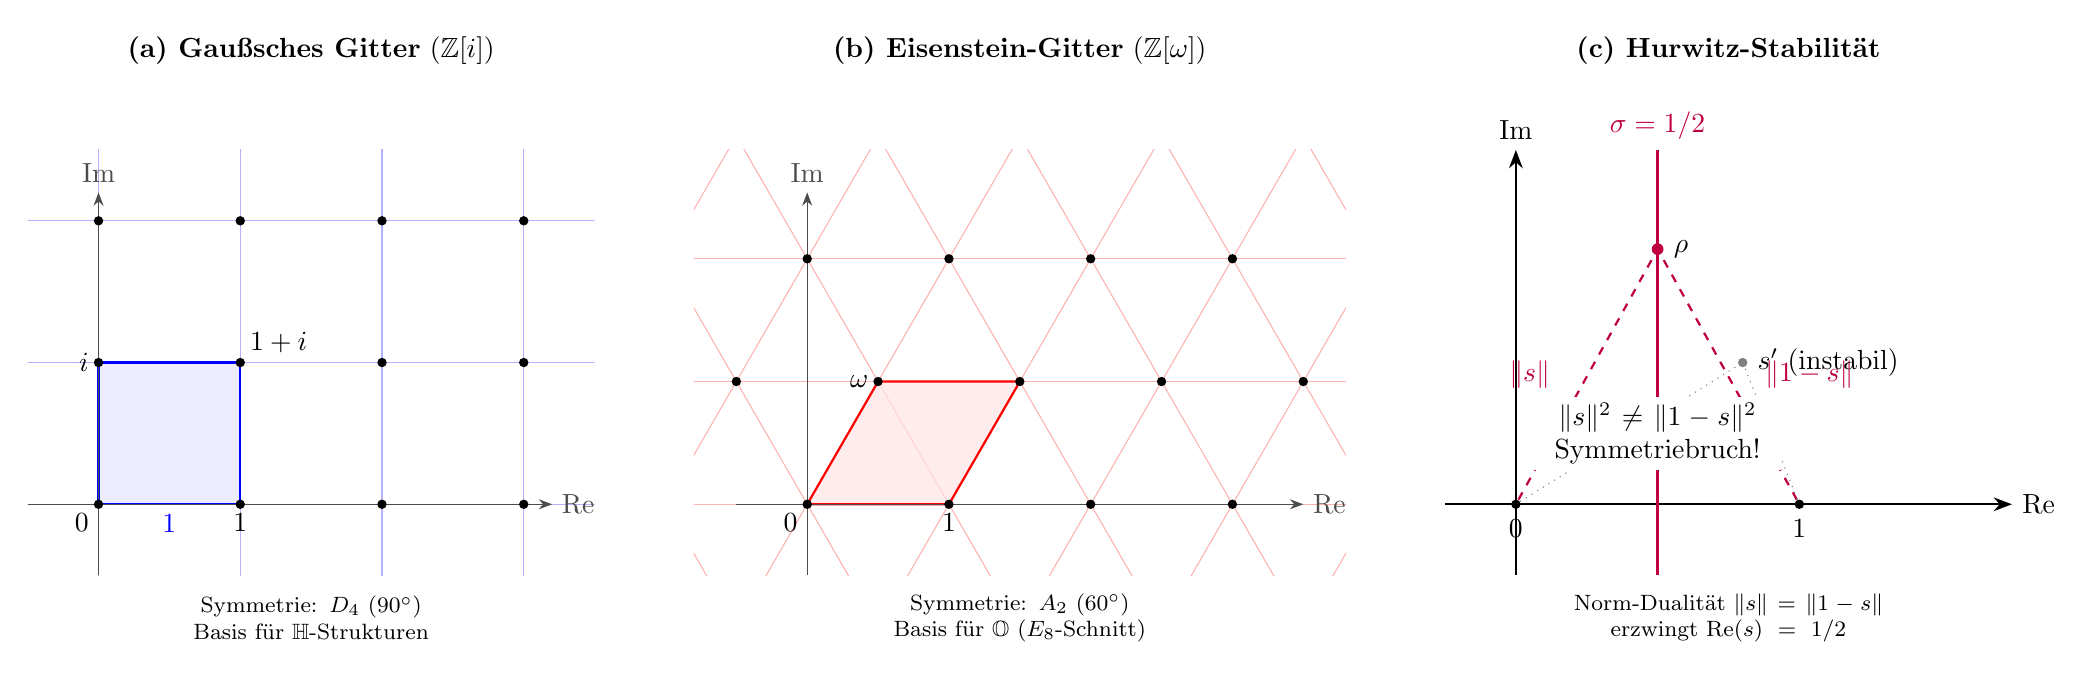
\begin{tikzpicture}[
    scale=1.8,
    >=Stealth,
    grid_node/.style={circle, fill=black, inner sep=1.2pt},
    gauss_line/.style={blue!30, thin},
    eisen_line/.style={red!30, thin},
    axis_line/.style={->, black!70, thin}
]

    % ======================================================================
    % PANEL A: GAUSS-GITTER (Quadratisch / D4 / Quaternionen-Slice)
    % ======================================================================
    \begin{scope}[local bounding box=gauss]
        \node at (1.5, 3.2) {\textbf{(a) Gaußsches Gitter} ($\mathbb{Z}[i]$)};
        \node[text width=4cm, align=center, font=\footnotesize] at (1.5, -0.8)
            {Symmetrie: $D_4$ ($90^\circ$)\\Basis für $\mathbb{H}$-Strukturen};

        % Grid
        \clip (-0.5, -0.5) rectangle (3.5, 2.5);
        \draw[step=1, gauss_line] (-1,-1) grid (4,4);

        % Fundamentalzelle
        \fill[blue!10, opacity=0.7] (0,0) rectangle (1,1);
        \draw[blue, thick] (0,0) -- (1,0) node[midway, below] {1} -- (1,1) -- (0,1) -- cycle;

        % Achsen
        \draw[axis_line] (-0.5,0) -- (3.2,0) node[right] {Re};
        \draw[axis_line] (0,-0.5) -- (0,2.2) node[above] {Im};

        % Punkte
        \foreach \x in {0,1,2,3}
            \foreach \y in {0,1,2}
                \node[grid_node] at (\x,\y) {};

        % Labels
        \node[below left] at (0,0) {0};
        \node[below] at (1,0) {1};
        \node[left] at (0,1) {$i$};
        \node[above right] at (1,1) {$1+i$};
    \end{scope}

    % ======================================================================
    % PANEL B: EISENSTEIN-GITTER (Hexagonal / E8-Slice / Oktonionen)
    % ======================================================================
    \begin{scope}[xshift=5cm, local bounding box=eisen]
        \node at (1.5, 3.2) {\textbf{(b) Eisenstein-Gitter} ($\mathbb{Z}[\omega]$)};
        \node[text width=4cm, align=center, font=\footnotesize] at (1.5, -0.8)
            {Symmetrie: $A_2$ ($60^\circ$)\\Basis für $\mathbb{O}$ ($E_8$-Schnitt)};

        % Clipping für sauberen Rand
        \clip (-0.8, -0.5) rectangle (3.8, 2.5);

        % sqrt(3)/2 für präzise hexagonal Koordinaten
        \pgfmathsetmacro{\sqrtThreeOverTwo}{0.8660254}

        % Gitter zeichnen (nur "nach vorne" um Überlappung zu vermeiden)
        \foreach \x in {-2,...,4} {
            \foreach \y in {-2,...,4} {
                \coordinate (P) at ({\x + 0.5*\y}, {\y * \sqrtThreeOverTwo});

                % Linien zu den drei Nachbarn in positiver Richtung
                \draw[eisen_line] (P) -- ++(1,0);
                \draw[eisen_line] (P) -- ++(0.5, \sqrtThreeOverTwo);
                \draw[eisen_line] (P) -- ++(-0.5, \sqrtThreeOverTwo);
            }
        }

        % Fundamentalzelle (Rhombus)
        \coordinate (O) at (0,0);
        \coordinate (A) at (1,0);
        \coordinate (B) at (1.5, \sqrtThreeOverTwo);   % 1 + omega
        \coordinate (C) at (0.5, \sqrtThreeOverTwo);   % omega

        \fill[red!10, opacity=0.7] (O) -- (A) -- (B) -- (C) -- cycle;
        \draw[red, thick] (O) -- (A) -- (B) -- (C) -- cycle;

        % Achsen
        \draw[axis_line] (-0.5,0) -- (3.5,0) node[right] {Re};
        \draw[axis_line] (0,-0.5) -- (0,2.2) node[above] {Im};

        % Punkte im sichtbaren Bereich
        \foreach \x in {-1,...,3}
            \foreach \y in {-1,...,3}
                \node[grid_node] at ({\x + 0.5*\y}, {\y * \sqrtThreeOverTwo}) {};

        % Labels
        \node[below left] at (0,0) {0};
        \node[below] at (1,0) {1};
        \node[left] at (0.5, \sqrtThreeOverTwo) {$\omega$};
    \end{scope}

    % ======================================================================
    % PANEL C: DER BEWEIS (GEOMETRIE)
    % ======================================================================
    \begin{scope}[xshift=10cm, local bounding box=proof]
        \node at (1.5, 3.2) {\textbf{(c) Hurwitz-Stabilität}};
        \node[text width=4.5cm, align=center, font=\footnotesize] at (1.5, -0.8)
            {Norm-Dualität $\|s\| = \|1-s\|$\\erzwingt $\text{Re}(s) = 1/2$};

        % Koordinatensystem (1 Einheit = 2cm für Lesbarkeit)
        \draw[->, thick] (-0.5,0) -- (3.5,0) node[right] {Re};
        \draw[->, thick] (0,-0.5) -- (0,2.5) node[above] {Im};

        % Punkte 0 und 1 (skaliert: 1 -> 2cm)
        \node[grid_node, label=below:0] (Z) at (0,0) {};
        \node[grid_node, label=below:1] (E) at (2,0) {};

        % Kritische Linie sigma = 1/2
        \draw[purple, very thick] (1, -0.5) -- (1, 2.5) node[above] {$\sigma = 1/2$};

        % Nullstelle rho auf der kritischen Linie
        \coordinate (Rho) at (1, 1.8);
        \node[circle, fill=purple, inner sep=1.5pt, label=right:$\rho$] at (Rho) {};

        % Gleichschenkliges Dreieck: ||s|| = ||1-s||
        \draw[purple, dashed, thick] (Z) -- (Rho) node[midway, left] {$\|s\| \quad$};
        \draw[purple, dashed, thick] (E) -- (Rho) node[midway, right] {$\quad \|1-s\|$};

        % Instabiler Punkt (Symmetriebruch)
        \coordinate (Wrong) at (1.6, 1.0);
        \node[circle, fill=gray, inner sep=1.2pt, label=right:$s'$ (instabil)] at (Wrong) {};
        \draw[gray, dotted] (Z) -- (Wrong);
        \draw[gray, dotted] (E) -- (Wrong);

        % Annotation
        \node[text width=3cm, align=center, fill=white, inner sep=2pt] at (1, 0.5)
            {$\|s\|^2 \neq \|1-s\|^2$\\Symmetriebruch!};
    \end{scope}

\end{tikzpicture}
\end{document}
